\documentclass[xcolor=dvipsnames, 14pt]{beamer}
\graphicspath{{./obr/}}
\usetheme[
		%english,
		%nameTitle,
		%tableOfContent,
        %numbering,
        ]{upolkgi}
%%\usetheme{Darmstadt}
%%\usecolortheme[named=LimeGreen]{structure}

% balíčky

%%\usepackage[utf8]{inputenc}
%%\usepackage[czech]{babel}
%%\usepackage{graphicx}

% informace o dokumentu
 \setbeamersize{text margin left=.5cm,text margin right=.5cm, text margin top=-2cm}
 \pdfcompresslevel=0
\begin{document}

\title[Synchronization and replication of geodata]{Synchronization and replication \\ of geodata in Esri platform}
\author[M. Solanská]{Markéta Solanská \\ supervisor: Doc. RNDr. Vilém Pechanec, Ph.D.}
\date[6.11.2013]{6.11.2013}


% text dokumentu


% titulní stránka
% (název prezentace, autor, datum...)

\begin{frame}
  \titlepage
\end{frame}

% osnova prezentace
% (většinou se pro délku vypouští)

% obsah prezentace
% (používají se klasické sekce)

\section{Synchronization and replication of geodata in Esri platform}

  \begin{frame}
    \frametitle{Main goals}
    \begin{itemize}
      \item store spatial data in a database system using ArcSDE technology and PostgreSQL
      \item replicate data between several datastores
    \end{itemize}
  \end{frame}
  
  \begin{frame}
    \frametitle{Main goals: Theoretical part}
    \begin{itemize}
      \item definition of terms: replication, synchronization, versioning
      \item description of replication possibilities, types and properties
      \item description of ArcSDE technology
      \item comparison of PostgreSQL and MS SQL Server Express replication possibilities and capabilities 
    \end{itemize}
  \end{frame}

  \begin{frame}
    \frametitle{Main goals: Practical part}
    \begin{itemize}
      \item set up replication of different data types
      \item solutions for various kinds of tasks
      \item test: performance, completeness, accuracy 
      \item RDBMSs: PostgreSQL 9.x + PostGIS, MS SQL Server Express 2008
      \item ESRI products: ArcSDE + ArcGIS for Desktop or ArcGIS for Server
    \end{itemize}
  \end{frame}

  \begin{frame}
    \frametitle{Replication}
    \begin{itemize}
      \item continuous copying of data from one server to another (one or more)
      \item full initial copy, then synchonization of changes
      \item main reasons for replication:
        \begin{itemize}
        \begin{normalsize}
          \item high availability
          \item load balancing
          \item data movement
          \item backing up without overloading master server
        \end{normalsize}
        \end{itemize}
    \end{itemize} 
  \end{frame}

%  \begin{frame}
%    \frametitle{Replication}
%    \begin{itemize}
%      \item master-slave replication
%      \\  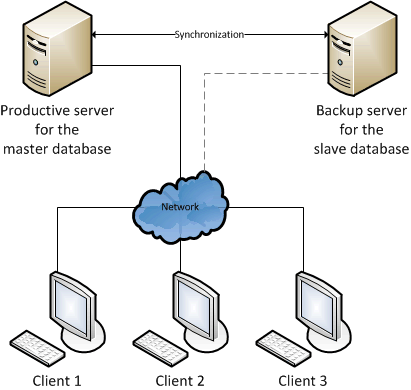
\includegraphics[scale=0.5]{obr/db_replikation.png} 
%      \\  \begin{tiny}(zdroj:http://www.passwordsafe.de/uploads/pics/db\_replikation\_EN.gif)\end{tiny}
%    \end{itemize} 
%  \end{frame}

  \begin{frame}
    \frametitle{ArcSDE Technology}
    \framesubtitle{ESRI product}
    \begin{itemize}
        \item middleware for communication between ArcGIS and SQL server (e.g. PostgreSQL)
        \item provides:
        \begin{itemize}
          {\normalsize 
            \item alternative method of ArcGIS spatial data storage (to RDBMS instead of filesystem)
            \item its own spatial data types
            \item its own replication solution 
          }
        \end{itemize} 
        \item enables multi-user editation
    \end{itemize} 
  \end{frame}

  \begin{frame}
    \frametitle{Already done}
    \begin{itemize}
      \item set up replication between two servers: 
        \\ both WIN XP/Linux Ubuntu + PostgreSQL(PostGIS) + Slony-I
      \item visualize in QuantumGIS
      \item test using simple vector data 
    \end{itemize}
  \end{frame}

  \begin{frame}
    \frametitle{To be done}
    \begin{itemize}
      \item test it for big amount of data
      \item visualization in ArcGIS
      \item use ArcSDE for connection to database
      \item set up replication using ArcSDE
      \item test the process of replication
      \item find solutions to different kinds of tasks
    \end{itemize}
  \end{frame}

  \begin{frame}
    \frametitle{Results}
    \begin{itemize}
      \item description of replication processes and related requirements of Esri products
      \item replication configuration instructions
      \item evaluation of reliability and performance of replication 
    \end{itemize}
  \end{frame}
  
  \begin{frame}
    \begin{center}
      {\Large\color{GisLightBlue}Thank you for your attention.}
    \end{center}
  \end{frame}
\end{document}
